\begin{applicationActivities}

\begin{activity}{5}
Consider a forest of bamboo that grows unimpeded by other organisms.  Which ODE models the size of the population best (all constants are positive)?
\vfill
\begin{enumerate}[(a)]
\item \(\frac{dB}{dt} = k\)
\item \(\frac{dB}{dt} = kB\)
\item \(\frac{dB}{dt} = kB-aB^2\)
\item \(\frac{dB}{dt} = kB^2\)
\end{enumerate}
\end{activity}

\begin{activity}{5}
The model \[\frac{dB}{dt}=kB\] models an ideal growth, free from competition (e.g. if population is sparse).

\vfill
The model \[ \frac{dB}{dt}=kB-aB^2\] models competitive growth.

\vfill
Observe that both models are autonomous.  Draw a phase line for each model, and describe the possible long term behaviors.
\end{activity}

\begin{activity}{10}
Which of the following best models the bamboo population in the presence of a panda population (\(P\))?
\vfill
\begin{enumerate}[(a)]
\item \(\frac{dB}{dt} = kB-aB^2\)
\item \(\frac{dB}{dt} = kB-aB^2-cP\)
\item \(\frac{dB}{dt} = kB-aB^2-cP^2\)
\item \(\frac{dB}{dt} = kB-aB^2-cBP\)
\end{enumerate}
\end{activity}

\begin{activity}{5}
Which of the following best models the (sparse) Panda population in the bamboo forest?
\vfill
\begin{enumerate}[(a)]
\item \(\frac{dP}{dt} = -dP \)
\item \(\frac{dP}{dt} = -dP+fBP \)
\item \(\frac{dP}{dt} = -dP-fBP \)
\item \(\frac{dP}{dt} = -dP-fBP-gP^2 \)
\end{enumerate}
\end{activity}

\begin{observation}
The interacting bamboo and Panda populations are modelled by the \term{autonomous system}
\begin{alignat*}{2}
\frac{dB}{dt} &= kb-aB^2-cBP\\
\frac{dP}{dt} &= -dP+fBP \\
\end{alignat*}

\vfill
These are referred to as \term{Lotka-Volterra equations}
\end{observation}

\begin{activity}{10}
Consider our Panda-Bamboo system
\begin{alignat*}{2}
\frac{dB}{dt} &= kB-aB^2-cBP\\
\frac{dP}{dt} &= -dP+fBP \\
\end{alignat*}
\begin{subactivity}
When is \(\frac{dB}{dt}\) zero?
\end{subactivity}
\begin{subactivity}
When is \(\frac{dP}{dt}\) zero?
\end{subactivity}
\end{activity}

\begin{observation}
These lines where the population of one species is unchanging are called \term{isoclines}

\begin{center}
\begin{tikzpicture}[scale=0.5]
\draw[->] (0,0) -- (10,0);
\node at (10.5,0) {\(B\)};
\draw[->] (0,0) -- (0,10);
\node at (0,10.5) {\(P\)};
\draw[thick,red] (5,0) -- (5,10);
\node at (5,-0.5) {\(\frac{d}{f}\)};
\draw[thick,red] (7,0) -- (0,6);
\node at (7,-0.6) {\(\frac{k}{a}\)};
\node at (-0.6,6) {\(\frac{k}{c}\)};
\end{tikzpicture}
\end{center}

\end{observation}

\begin{activity}{15}
\begin{center}
\begin{tikzpicture}[scale=0.4]
\draw[->] (0,0) -- (10,0);
\node at (10.5,0) {\(B\)};
\draw[->] (0,0) -- (0,10);
\node at (0,10.5) {\(P\)};
\draw[thick,red] (5,0) -- (5,10);
\node at (5,-0.5) {\(\frac{d}{f}\)};
\draw[thick,red] (7,0) -- (0,6);
\node at (7,-0.6) {\(\frac{k}{a}\)};
\node at (-0.6,6) {\(\frac{k}{c}\)};
\node[blue] at (7,4) {1};
\node[blue] at (3,5) {2};
\node[blue] at (2,2) {3};
\node[blue] at (5.5,0.5) {4};
\end{tikzpicture}
\end{center}
For each of the four regions
\begin{subactivity}
Determine if each of \(\frac{dP}{dt}\) and \(\frac{dB}{dt}\) is positive or negative.
\end{subactivity}
\begin{subactivity}
Determine the general direction of a solution curve (\term{trajectory}) in that region (e.g. up and right).
\end{subactivity}
\begin{subactivity}
Describe the general shape of the trajectories.
\end{subactivity}
\end{activity}

\begin{observation}
Plotting the slope field  with software makes it more clear that the trajectories are closed curves.
\begin{center}
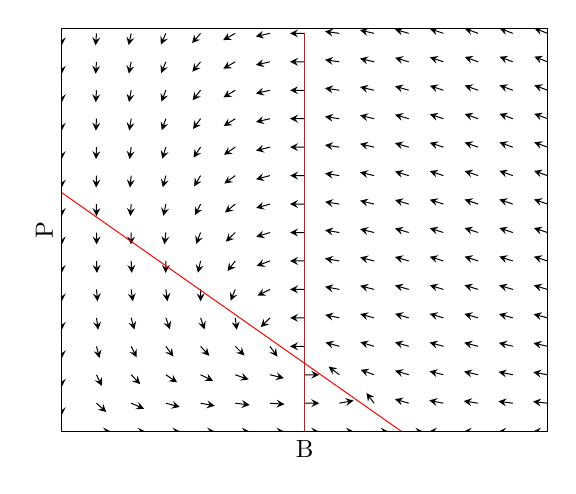
\begin{tikzpicture}[scale=0.9]
    \begin{axis}[
        domain=0:10,
        view={0}{90},
        axis background/.style={fill=white},
		yticklabels={,,},
		xticklabels={,,},
		xlabel={B},
		ylabel={P},
		ticks=none,
    ]
        \addplot3[black,
            quiver={
             u={1.5*(x-0.14*x^2-0.167*x*y)/sqrt(  (x-0.14*x^2-0.167*x*y)^2+  (-y+0.2*x*y)^2)  },
             v={1.5*(-y+0.2*x*y)/sqrt(  (x-0.14*x^2-0.167*x*y)^2+  (-y+0.2*x*y)^2)},
             scale arrows=0.2,
            },
            -stealth,samples=15]
                {exp(-x) - 1/2*sin(x) - 1/2*cos(x)};
		\addplot[red] coordinates {(5,0) (5,10)};
		\addplot[red] coordinates {(7,0) (0,6)};
    \end{axis}

\end{tikzpicture}
\end{center}
\end{observation}


\end{applicationActivities}
